\documentclass[aspectratio=169,
hyperref={colorlinks,urlcolor=blue}
]{beamer}


%\usetheme{Pittsburgh}
\usetheme{default}
\usepackage{colortbl}%colored tables
%For using helvetica font:
\usepackage[scaled]{helvet}
\usepackage[T1]{fontenc}
\renewcommand\familydefault{\sfdefault}
\urlstyle{same} %sets the fonts for urls
\usepackage{pdfpages}
\usepackage{siunitx}
\usepackage{caption}
\usepackage{pifont}%for dings
\usepackage{pgfplots}%for 3d plotting
\pgfplotsset{compat = newest}
\usepackage{mathtools}%box in align env \Aboxed
\usepackage[american,smartlabels]{circuitikz}%for drawing circuits
\usepackage{multimedia}
\usepackage{animate}
\usepackage{xcolor}


\usetikzlibrary{arrows}
\usetikzlibrary {3d} 
\usetikzlibrary{decorations.markings, math}
\usetikzlibrary{intersections, pgfplots.fillbetween}
\usetikzlibrary {shapes.geometric} 


%\definecolor{myblue}{RGB}{5, 34, 150}
\definecolor{myblue2}{RGB}{5, 34, 150}
\definecolor{myblue}{RGB}{0,36,82}
\definecolor{myred}{RGB}{207, 2, 13}
\definecolor{mygreen}{RGB}{0, 158, 11}
\definecolor{myyellow}{RGB}{220,220,0}
\definecolor{qblue}{RGB}{0,36,82}
\definecolor{qgold}{RGB}{250,189,15}
\definecolor{qred}{RGB}{185,14,49}
\definecolor{cblue}{rgb}{0.13, 0.67, 0.8}
\definecolor{corange}{rgb}{0.8, 0.34, 0.0}
\definecolor{cpurple}{rgb}{0.54, 0.29, 0.42}

%%%%%%%%%%%% General settings
\setbeamercolor{frametitle}{fg=black}
\setbeamercolor{title}{fg=black}
\setbeamercolor{author}{fg=myblue2}

\beamertemplatenavigationsymbolsempty %no navigation controls at bottom of slides
%\setbeamertemplate{footline}[frame number]
\usefonttheme{professionalfonts} 
\setbeamerfont{title}{series=\bfseries,parent=structure}
\setbeamerfont{frametitle}{series=\bfseries,parent=structure}

%%%%%%%%%%%%Lists
\setbeamertemplate{itemize item}[circle] %{\color{myblue}$\circ$}
\setbeamertemplate{itemize subitem}{\color{myblue2}$\circ$}
\setbeamertemplate{itemize subsubitem}{\color{myblue2}$\cdot$}
\setbeamercolor{itemize item}{bg=myblue2,fg=myblue2}
\setbeamercolor{enumerate item}{bg=myblue2,fg=myblue2}
%%%%%%%%%%%%%%%%%%%%%%%%%%%%

%%%%%%%%%%%%Blocks
\setbeamertemplate{blocks}[rounded]
%Default block
\setbeamercolor{block title}{bg=myblue2, fg=white}
\setbeamercolor{block body}{bg=myblue2!10}
\setbeamerfont{block body}{size=\scriptsize}
\setbeamerfont{block title}{size=\scriptsize}
%Alert block
\setbeamercolor{block title alerted}{bg= myblue2, fg=white}
\setbeamercolor{block body alerted}{bg=myblue2!10}
\setbeamerfont{block body alerted}{size=\scriptsize}
\setbeamerfont{block title alerted}{size=\scriptsize}
%example block
\setbeamercolor{block title example}{bg=mygreen, fg=white}
\setbeamercolor{block body example}{bg=mygreen!10}
\setbeamerfont{block body example}{size=\scriptsize}
\setbeamerfont{block title example}{size=\scriptsize}
%%%%%%%%%%%%%%%%55


%%%%%%%%%%%%Figures and captions
\captionsetup{font=scriptsize,labelfont=scriptsize}
%\setbeamertemplate{caption}{\raggedright\insertcaption\par}
\newenvironment{capfig}[3]{\begin{figure}\includegraphics[width=#1\textwidth]{#2}\caption*{\textit{#3}}\end{figure}}{}

%\makeatother
%\setbeamertemplate{footline}
%{
%  \leavevmode%
%  \hbox{%
%  \begin{beamercolorbox}[wd=.4\paperwidth,ht=2.25ex,dp=1ex,center]{author in head/foot}%
%    \usebeamerfont{author in head/foot}\insertshortauthor
%  \end{beamercolorbox}%
%  \begin{beamercolorbox}[wd=.6\paperwidth,ht=2.25ex,dp=1ex,center]{title in head/foot}%
%    \usebeamerfont{title in head/foot}\insertshorttitle\hspace*{3em}
%    \insertframenumber{} / \inserttotalframenumber\hspace*{1ex}
%  \end{beamercolorbox}
%  }%
%  \vskip0pt%
%}
%\makeatletter

\makeatother
\setbeamertemplate{footline}
{
  \leavevmode%
  \hbox{%
\begin{beamercolorbox}[wd=.27\paperwidth,ht=2.25ex,dp=1ex,center]{author in head/foot}%
    \color{black}{\insertinstitute}
\end{beamercolorbox}
  \begin{beamercolorbox}[wd=.27\paperwidth,ht=2.25ex,dp=1ex,center]{author in head/foot}%
    \color{black}{\inserttitle}
  \end{beamercolorbox}%
  \begin{beamercolorbox}[wd=.27\paperwidth,ht=2.25ex,dp=1ex,center]{title in head/foot}%
    \color{black}{\insertshortauthor}
  \end{beamercolorbox}
  \begin{beamercolorbox}[wd=.27\paperwidth,ht=2.25ex,dp=1ex,center]{title in head/foot}%
    \hspace{.28\paperwidth}\color{black} \insertframenumber{} / \inserttotalframenumber\hspace*{1ex}
  \end{beamercolorbox}
  }%
  \vskip0pt%
}
\makeatletter

\setbeamertemplate{title page}
{
  \begin{tikzpicture}[remember picture,overlay]
    \def\barh{4}%15
  
    \draw[color=myblue2,line width=\barh] ([yshift=-0.5*\barh]current page.north west) -- ([yshift=-0.5*\barh,xshift=-0.67\paperwidth]current page.north east);
    \draw[color=myblue2,line width=\barh] ([yshift=-0.5*\barh,xshift=-0.67\paperwidth]current page.north east) -- ([yshift=-0.5*\barh,xshift=-0.34\paperwidth]current page.north east);
    \draw[color=myblue2,line width=\barh] ([yshift=-0.5*\barh,xshift=-0.34\paperwidth]current page.north east) -- ([yshift=-0.5*\barh]current page.north east); 
  
    \draw[color=myblue2,line width=\barh] ([yshift=0.5*\barh]current page.south west) -- ([yshift=0.5*\barh,xshift=-0.67\paperwidth]current page.south east);
    \draw[color=myblue2,line width=\barh] ([yshift=0.5*\barh,xshift=-0.67\paperwidth]current page.south east) -- ([yshift=0.5*\barh,xshift=-0.34\paperwidth]current page.south east);
    \draw[color=myblue2,line width=\barh] ([yshift=0.5*\barh,xshift=-0.34\paperwidth]current page.south east) -- ([yshift=0.5*\barh]current page.south east);
    %\node[left] at (current page.east) {
    %
\includegraphics[scale=0.1]{figures/coverpage}
    %};
  \end{tikzpicture}
  
  \usebeamerfont{title}\usebeamercolor[fg]{title}\inserttitle\par
  \usebeamerfont{subtitle}\usebeamercolor[fg]{subtitle}\insertsubtitle\par
  \vspace{2cm}
  \usebeamerfont{author}\usebeamercolor[fg]{author}\insertauthor\par
  \usebeamerfont{institute}\usebeamercolor[fg]{author}\insertinstitute\par
  \usebeamercolor[fg]{author}\par
  \usebeamercolor[fg]{titlegraphic}\inserttitlegraphic

} 

\setbeamertemplate{frametitle}{%
    \nointerlineskip%
        \par\hspace*{-\dimexpr0.5\paperwidth-0.5\textwidth}\textcolor{myblue2}{\rule{0.33\paperwidth}{6pt}}\textcolor{myblue2}{\rule{0.33\paperwidth}{6pt}}\textcolor{myblue2}{\rule{0.34\paperwidth}{6pt}} 
    \begin{beamercolorbox}[wd=\paperwidth,ht=0.75cm,dp=0.6ex]{frametitle}
        \hspace*{0.5cm}\strut\usebeamerfont{frametitle}\insertframetitle\strut
        %\hrule
    \end{beamercolorbox}%
    %%Line below:
%\par\hspace*{-\dimexpr0.5\paperwidth-0.5\textwidth}\textcolor{myblue}{\rule{\paperwidth}{0.4pt}}
     % <-- calculation of left margin width + rule
     %\textcolor{red}{\noindent\rule{\paperwidth}{2pt}}
}


%%%%%%%%%%%%Frame templates

%Slide with title
\newenvironment{titleframe}[1]
{\begin{frame}\frametitle{#1}\end{frame}}
{}

%Slide with title and itemize list:
\newenvironment{bulletframe}[1]
{\begin{frame}{#1} \itemize}
{\enditemize \end{frame}}

%Slide with two columns 50/50
\newenvironment{twocolframe}[3]
{\begin{frame}{#1}
 \begin{columns}[T]
 \column{0.5\textwidth}#2
 \column{0.5\textwidth}#3
 \end{columns}\end{frame}}{}

%Slide with two columns 60/40 <<<<<<<<<<<<<<<<<<<<<<  This one!
\newenvironment{twocolframesf}[3]
{\begin{frame}{#1}
 \begin{columns}[T]
 \column{0.6\textwidth}#2
 \column{0.4\textwidth}#3
 \end{columns}\end{frame}}{}
 
%Slide with two columns 70/30
\newenvironment{twocolframest}[3]
{\begin{frame}{#1}
 \begin{columns}[T] 
 \column{0.7\textwidth}#2
 \column{0.3\textwidth}#3
 \end{columns}\end{frame}}{} 
 
%Slide with two columns 40/60
\newenvironment{twocolframefs}[3]
{\begin{frame}{#1}
 \begin{columns}[T] 
 \column{0.4\textwidth}#2
 \column{0.6\textwidth}#3
 \end{columns}\end{frame}}{}
 
%Slide with two columns 70/30
\newenvironment{twocolframets}[3]
{\begin{frame}{#1}
 \begin{columns}[T] 
 \column{0.3\textwidth}#2
 \column{0.7\textwidth}#3
 \end{columns}\end{frame}}{} 

 
%Colloquium speaker (title, abstract, picture file, speaker name)
\newenvironment{colloquium}[5]
{
\begin{frame}{Colloquium: Friday 1:30pm in Stirling A}
\begin{columns}[T] 
 \column{0.8\textwidth}
 \textbf{#1}\\
 #2
 \column{0.2\textwidth}
 \capfig{#3}{#4}{#5}
 \end{columns}
\end{frame}
}
{} 

%%%%%%%%%%%%%Set Hyperref colors


\hypersetup{
  colorlinks=true,
  linkcolor=blue,    
  urlcolor=blue,     
  citecolor=blue      
}
%%%%%%%%%%%%%TOC bolding
\setbeamerfont{section in toc}{series=\bfseries}



%Frames:
% \twocolframesf 60/40 (fs, st, ts) 
% \titleframe
% bulletframe


%%%%%%%%%%%%%%%%%%%%%%%%%
%%%%%% START OF PRESENTATION %%%%%%
%%%%%%%%%%%%%%%%%%%%%%%%%

\title{Momentum and Centre of Mass}
\subject{Systems, Collisions and Centre of Mass}
\subtitle{Building Models to Describe our World}


\begin{document}

%%%%%%%%%%%%%%%%%%%%%%%%%
%%%%%% Title slide %%%%%%
%%%%%%%%%%%%%%%%%%%%%%%%%
\chaptertitle{Momentum and Centre of Mass}
\begin{frame}
\titlepage
\thispagestyle{empty}

\begin{textblock*}{5cm}(11cm,4cm)
    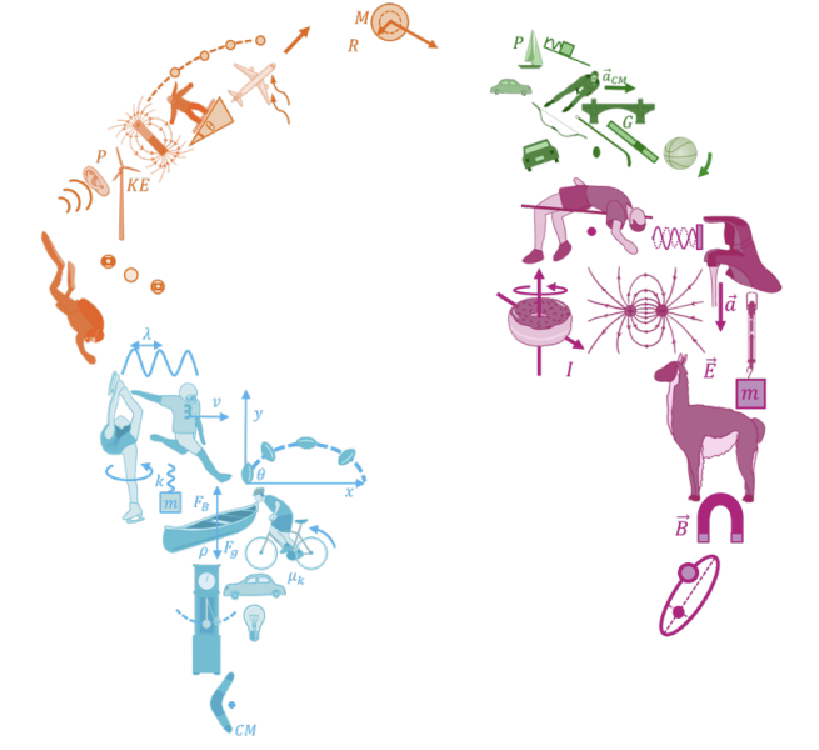
\includegraphics[width=4cm]{figures/BMDW/logo}
\end{textblock*}

\end{frame}

%%%%%%%%%%%%%TOC

\twocolframe{Outline}
{\tableofcontents[sections=1-2, subsectionstyle=show/show]\thispagestyle{empty}}
{\tableofcontents[sections=3, subsectionstyle=show/show]}

%%%%%%%%%%%%%%%%%%%%%%%%%









%%%%%%%%%%%%%%%%%%%%%%%%%%%%%%%%
\section{Momentum Basics}
\label{sec:momentumbasics}
\title{Momentum Basics}
\institute{Momentum and Centre of Mass}
\author{\insertsubsection}


%%%%%%%%%%%%%%%%%%%%%%%%%
\begin{frame}
\titlepage
\thispagestyle{empty}
\end{frame}

%%%%%%%%%%%%%%













%%%%%%%%%%%%%%%%%%%%%%%%%%%%
\subsection{Momentum of  a particle}
\label{subsec:momentumofaparticle}
\begin{frame}{Momentum of a particle}
\begin{itemize}
\item The momentum of a particle of mass $m$ is:
\begin{align*}
\vec p = m \vec v
\end{align*}
\item The rate of change of momentum is the net force on the particle:
\begin{align*}
\frac{d\vec p}{dt} &= \frac{d}{dt}m\vec v= m\frac{d\vec v}{dt} = m\vec a\\
\therefore \frac{d\vec p}{dt} &= \sum \vec F = \vec F^{net}
\end{align*}
\item \textbf{If the net force on a particle is zero, its momentum is constant} (it doesn't change with time).
\end{itemize}

\end{frame}


%%%%%%%%%%%%%%%%%%%%%%%%%%%%%%%%



%%%%%%%%%%%%%%%%%%%%%%%%%%%%%%%%
\subsection{Impulse}
\label{subsec:impulse}
\twocolframesf{Impulse}
{
\vspace{-0.5cm}
\begin{itemize}
\item The net impulse \textbf{vector} is the change in momentum:
\begin{itemize}
\item If force does not change with time:
\begin{align*}
\frac{d\vec p}{dt} &\sim\frac{\Delta \vec p}{\Delta t} =\vec F^{net}\\
\therefore \vec J^{net} &= \Delta \vec p=\vec F^{net} \Delta t
\end{align*}
\item If force changes magnitude or direction with time
\begin{align*}
\vec J^{net} = \Delta \vec p = \int_{t_a}^{t_b}\vec F^{net}(t) dt
\end{align*}
\end{itemize}
\item A force acting for a given time will change the momentum.
\item \textit{What makes it different from Work}?
\end{itemize}
}
{
\begin{center}
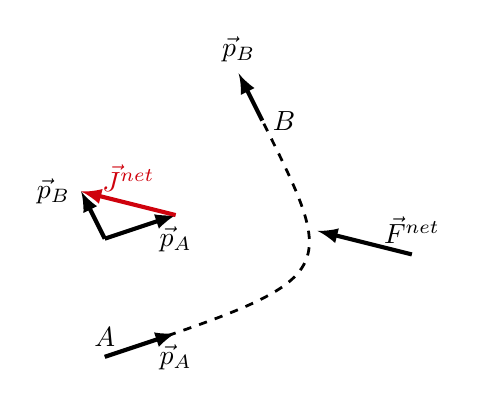
\begin{tikzpicture}
\tikzmath{
\L=2;
\h=3;
}
\scalebox{1}{
\coordinate (P1) at (0,0);
\coordinate (C1) at (\h,\L/2);
\coordinate (P2) at (\L,\h);

\draw[line width=1, dashed] (P1) node[above]{$A$} .. controls (C1) .. (P2) node[right]{$B$};
\draw[-latex, line width =1.5] (P1) -- ($(P1)!0.3!(C1)$) node[below]{$\vec p_A$};
\draw[-latex, line width =1.5] (P2) -- ($(P2)!-0.3!(C1)$) node[above]{$\vec p_B$};

\begin{scope}[shift={(0,1.5)}]

\draw[-latex, line width =1.5] (0,0) -- ($(0,0)!0.3!(\h,\L/2)$) node[below]{$\vec p_A$};
\draw[-latex, line width =1.5, color=myred] ($(0,0)!0.3!(\h,\L/2)$) -- ($ (\L,\h)!-0.3!(\h,\L/2)-(\L,\h)$) node[midway,above]{$\vec J^{net}$};
\end{scope}

\begin{scope}[shift={(-\L,1.5-\h)}]
\draw[-latex, line width =1.5] (\L,\h) -- ($(\L,\h)!-0.3!(\h,\L/2)$) node[left]{$\vec p_B$};
\end{scope}

\begin{scope}[shift={(\h,\L/2)}]
\draw[-latex, line width =1.5] ($(0,0)!0.3!(\h,\L/2)$)node[above]{$\vec F^{net}$} -- ($ (\L,\h)!-0.3!(\h,\L/2)-(\L,\h)$) ;
\end{scope}

}
\end{tikzpicture}
\captionof*{figure}{\textit{Impulse is the change in momentum.}}
\end{center}
\begin{align*}
\vec J^{net}=\Delta \vec p=\vec p_B-\vec p_A = \vec F^{net}\Delta t
\end{align*}
}


%%%%%%%%%%%%%%%%%%%%%%%%%%%%%%%%


%%%%%%%%%%%%%%%%%%%%%%%%%%%%%%%%
\subsection{Systems of particles}
\label{subsec:systemsofparticles}
\begin{frame}{Systems of particles}
\begin{itemize}
\item Newton’s Second Law is only valid for a point particle (an infinitely small particle of mass, $m$).
\item Loosely, we call a collection of particles a ``system''.
\item A solid block of matter is a system of many particles that cannot move relative to each other.
\item A gas is a system of many particles that can move relative to each other.
\item So far, we have modelled, say, blocks and treated them like point particles even if they are not.
\item We can distinguish between ``internal'' and ``external'' forces to the system.
\end{itemize}
\end{frame}


%%%%%%%%%%%%%%%%%%%%%%%%%%%%%%%%


%%%%%%%%%%%%%%%%%%%%%%%%%%%%%%%%
\twocolframesf{Modeling 2 blocks as a system}
{
\only<1>{
\begin{itemize}
\item Want to know the acceleration of the two blocks, given $F$, friction.
\item Can apply Newton's Second Law to each block (4 equations, blocks have the same acceleration):
\begin{align*}
\sum F_1^{horiz}&=T-\mu_k N_1=m_1a\\
\sum F_2^{horiz}&=F-T-\mu_k N_2=m_2a\\
&+\text{forces in vertical direction}
\end{align*}
\end{itemize}
}
\only<2>{
\begin{itemize}
\item But, the motion of the system, $(m_1+m_2)$, depends on the external forces on the system. Tension is an \textit{internal} force.
\item Consider adding together Newton’s Second Law for each particle:
\begin{align*}
\sum F_1^{horiz}=T-\mu_k N_1&=m_1a\\
\sum F_2^{horiz}=F-T-\mu_k N_2&=m_2a\\
\sum F_1^{horiz} + \sum F_2^{horiz}&=\textcolor{myred}{T}-\mu_k N_1+F\textcolor{myred}{-T}-\mu_k N_2\\
\therefore F-\mu_k(N_1+N_2)&=(m_1+m_2)a\\
F-\mu_k(m_1+m_2)g&=(m_1+m_2)a
\end{align*}
\end{itemize}
}
}
{
\begin{center}
\vspace{-1cm}
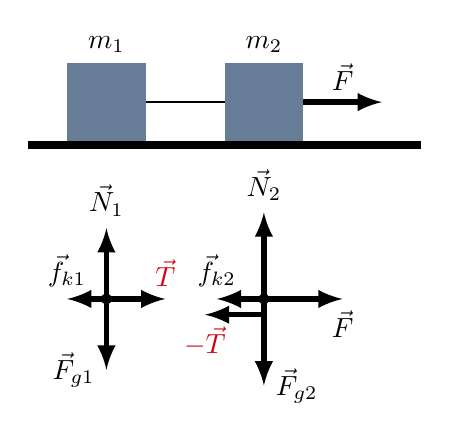
\begin{tikzpicture}
\tikzmath{
\L=5;
\abox=1;
}

\scalebox{1}{
\fill (0,-0.1) rectangle (\L,0);

\fill[color=myblue!60] (0.5,0) rectangle +(\abox,\abox);
\fill[color=myblue!60] (2.5,0) rectangle +(\abox,\abox);
\node[above] at (0.5+\abox/2,\abox) {$m_1$};
\node[above] at (2.5+\abox/2,\abox) {$m_2$};
\draw[line width=1] (0.5+\abox,\abox/2) -- +(1,0);
\draw[-latex,line width=2] (2.5+\abox,\abox/2) -- +(1,0) node[midway,above]{$\vec F$};

\begin{scope}[shift={(0,-3)}]
\coordinate (P1) at (0.5+\abox/2,\abox);
\coordinate (P2) at (2.5+\abox/2,\abox);

\fill (P1) circle (2pt);
\fill (P2) circle (2pt);

\draw[-latex, line width=2] (P1) -- +(-0.5,0) node[above]{$\vec f_{k1}$};
\draw[-latex, line width=2] (P2) -- +(-0.6,0) node[above]{$\vec f_{k2}$};

\draw[-latex, line width=2] (P1) -- +(0.75,0) node[above]{$\textcolor{myred}{\vec T}$};
\draw[-latex, line width=2] ($(P2)-(0,0.2)$) -- +(-0.75,0) node[below]{$\textcolor{myred}{-\vec T}$};
\draw[-latex, line width=2] ($(P2)$) -- +(1,0) node[below]{$\vec F$};

\draw[-latex, line width=2] (P1) -- +(0,0.9) node[above]{$\vec N_{1}$};
\draw[-latex, line width=2] (P2) -- +(0,1.1) node[above]{$\vec N_{2}$};

\draw[-latex, line width=2] (P1) -- +(0,-0.9) node[left]{$\vec F_{g1}$};
\draw[-latex, line width=2] (P2) -- +(0,-1.1) node[right]{$\vec F_{g2}$};

\end{scope}

}
\end{tikzpicture}
\captionof*{figure}{\textit{Modeling two connected blocks, either individually or as a system.}}
\end{center}
\only<2>{
\scriptsize
The internal forces (exerted by one object of the system on another) always cancel out because of Newton’s Third Law. Only the external forces affect the motion of the system.
}
}


%%%%%%%%%%%%%%%%%%%%%%%%%%%%%%%%
\subsection{Momentum of a system}
\label{subsec:momentumofasystem}
\begin{frame}{Momentum of a system}
\begin{itemize}
\item If many particles make up a system, we can add their individual momenta together to define the total momentum of the system:
\begin{align*}
\vec P = \vec p_1 + \vec p_2 +\vec p_3+\dots
\end{align*}
\item The rate of change of momentum of the system is given by the sum of the \textbf{external forces} exerted on the system:
\begin{align*}
\frac{d\vec P}{dt}=\frac{d\vec p_1}{dt} + \frac{d\vec p_2}{dt}  + \frac{d\vec p_3}{dt} +\dots=  \sum \vec F ^{ext}
\end{align*}
\item If there is \textbf{no net external force on the system, the momentum of the system is conserved}.
\end{itemize}
\end{frame}


%%%%%%%%%%%%%%%%%%%%%%%%%%%%%%%%








%%%%%%%%%%%%%%%%%%%%%%%%%%%%%%%%
\section{Collisions}
\label{sec:collisions}
\title{Collisions}
\institute{Momentum and Centre of Mass}
\author{\insertsubsection}


%%%%%%%%%%%%%%%%%%%%%%%%%
\begin{frame}
\titlepage
\thispagestyle{empty}
\end{frame}

%%%%%%%%%%%%%%











%%%%%%%%%%%%%%%%%%%%%%%%%%%%%%%%
\subsection{Concept}
\label{subsec:collisionconcept}
\twocolframesf{Collisions}
{
\begin{itemize}
\item ``Events'' where one considers the total momentum of a system ``just before'' and ``just after''.
\item Examples:
\begin{itemize}
\item Billiard balls colliding.
\item An arrow embedding itself into a block of wood that can move.
\item A bomb exploding into fragments.
\end{itemize}
\item Even if there are net external forces (e.g. gravity), one can \textbf{usually} neglect them if the momentum is compared just before and just after the collision and model total momentum as being conserved.
\end{itemize}
}
{
\begin{center}
\begin{tikzpicture}
\tikzmath{
\L=5;
\h=\L/2;
\w=6;
}

\scalebox{1}{
%table
\fill[color=poolgreen, draw=brown, line width=5pt] (0,0) rectangle (\L,\h);
%pockets
\fill (0,0) circle(3pt);.
\fill (0,\h) circle(3pt);
\fill (\L/2,0) circle(3pt);
\fill (\L/2,\h) circle(3pt);
\fill (\L,0) circle(3pt);
\fill (\L,\h) circle(3pt);
%balls
\shade[ball color=white,opacity=0.5] (\L/2-0.4,\h/2) circle(2.5pt);
\shade[ball color=white,opacity=0.6] (\L/2-0.25,\h/2) circle(2.5pt);
\shade[ball color=white,opacity=0.7] (\L/2-0.15,\h/2) circle(2.5pt);
\shade[ball color=white] (\L/2,\h/2) circle(2.5pt);

\shade[ball color=black,opacity=0.3] (\L/2+0.2,\h/2+0.1) circle(2.5pt);
\shade[ball color=black,opacity=0.4] (\L/2+0.4,\h/2+0.2) circle(2.5pt);
\shade[ball color=black,opacity=0.5] (\L/2+0.6,\h/2+0.3) circle(2.5pt);
\shade[ball color=black] (\L/2+0.8,\h/2+0.4) circle(2.5pt);

\shade[ball color=purple,opacity=0.3] (\L/2+0.2,\h/2-0.1) circle(2.5pt);
\shade[ball color=purple,opacity=0.4] (\L/2+0.3,\h/2-0.2) circle(2.5pt);
\shade[ball color=purple,opacity=0.5] (\L/2+0.4,\h/2-0.3) circle(2.5pt);
\shade[ball color=purple] (\L/2+0.5,\h/2-0.4) circle(2.5pt);
}
\end{tikzpicture}
\captionof*{figure}{\textit{Billiard balls colliding.}}
\end{center}

\begin{center}
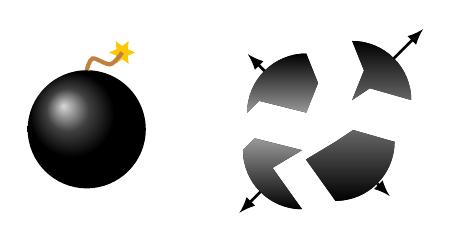
\begin{tikzpicture}
\tikzmath{
\R=0.75;
}

\scalebox{1}{
\shade[ball color=black] (0,0) circle(\R);
\node [star, star points=6, star point ratio=0.5, minimum size=0.05cm, fill=yellow!60!orange]
       at (0.6*\R,1.3*\R){};
\draw[line width=1.5pt, color=brown] plot [smooth] coordinates {(0,\R) (0.1*\R,1.2*\R)  (0.4*\R,1.1*\R) (0.6*\R,1.3*\R) };

\begin{scope}[shift={(3cm,0)}]
%\draw (45:1.2*\R) circle(4pt);

\fill[top color=black, bottom color=black!60] (45:0.7*\R) -- ($(45:0.7*\R)+(0.3*\R,0.2*\R)$) -- ($(45:0.7*\R)+(\R,0)$) arc(0:90:\R) -- ($(45:0.7*\R)+(0.2*\R,0.5*\R)$) --cycle ;
\fill[top color=black, bottom color=black!40] (135:0.4*\R) -- ($(135:0.4*\R)+(0.2*\R,0.5*\R)$) -- ($(135:0.4*\R)+(0,\R)$) arc(90:180:\R) -- ($(135:0.4*\R)+(-0.8*\R,0.2*\R)$)--cycle ;
\fill[bottom color=black, top color=black!40] (225:0.5*\R) -- ($(225:0.5*\R)+(-0.8*\R,0.2*\R)$) -- ($(225:0.5*\R)+(-\R,0)$) arc(180:270:\R) -- ($(225:0.5*\R)+(-0.5*\R,-0.3*\R)$)  --cycle;
\fill[bottom color=black, top color=black!60] (315:0.3*\R) -- ($(315:0.3*\R)+(-0.5*\R,-0.3*\R) $) -- ($(315:0.3*\R)+(0,-\R) $)arc(-90:0:\R) -- ($(315:0.3*\R)+(0.3*\R,0.2*\R) $)  --cycle ;

\draw [-latex, line width=1] (45:1.7*\R) -- +(45:0.7*\R);
\draw [-latex, line width=1] (135:1.4*\R) -- +(135:0.4*\R);
\draw [-latex, line width=1] (225:1.5*\R) -- +(225:0.5*\R);
\draw [-latex, line width=1] (315:1.3*\R) -- +(315:0.3*\R);

\end{scope}


}
\end{tikzpicture}
\captionof*{figure}{\textit{An explosion.}}
\end{center}
}

%%%%%%%%%%%%%%%%%%%%%%%%%%%%%%%%


%%%%%%%%%%%%%%%%%%%%%%%%%%%%%%%%
\subsection{Elastic vs inelastic}
\label{subsec:elasticvinelastic}
\begin{frame}{Elastic vs Inelastic}
\begin{itemize}
\item Just because momentum is conserved does not mean that mechanical energy is conserved:
\begin{itemize}
\item \textbf{Momentum }is conserved when there is \textbf{no net external force} on the system.
\item \textbf{Energy} is conserved when there is \textbf{no non-conservative force} doing work on any particle in the system.
\end{itemize}
\item To model elastic collisions, the mechanical energy of the system is conserved before and after the collision:
\begin{align*}
E=K+U=K'+U'=E'
\end{align*}
\item $K$, $U$ are the total kinetic energy and total potential energy of the system (add together the kinetic and potential energies of all particles in the system).
\item Usually, if the collision happens over a small distance, then the potential energies are (almost) the same before and after the collision (potential energy depends on position and if position doesn’t change much, neither does $U$):
\begin{align*}
U=U'\quad \text{(Usually)}
\end{align*}
\end{itemize}
\end{frame}


%%%%%%%%%%%%%%%%%%%%%%%%%%%%%%%%
\subsection{Elastic collision in 1D}
\label{subsec:elasticcollisionin1d}
\twocolframesf{Elastic collision in 1D: $m$ collides with $m$ at rest}
{
\vspace{-0.25cm}
\begin{itemize}
\item<1-> Conservation of momentum:
\begin{align*}
m\vec v_1=m\pvec v_1'+m \pvec v_2'
\end{align*}
\item<2-> $x$-component:
\begin{align*}
 \Aboxed{v_1= v_1'+v_2'}
\end{align*}
\item<3-> Conservation of energy:
\begin{align*}
\frac{1}{2}mv_1^2&=\frac{1}{2}m{v'}_1^{2}+\frac{1}{2}m{v'}_2^{2}\\
\therefore \Aboxed{v_1^2&= {v'}_1^{2}+ {v'}_2^{2}}
\end{align*}
\item<3-> 2 equations 2 unknowns, but not trivial, since not linear (i.e. quadratic)
\end{itemize}
}
{
\begin{center}
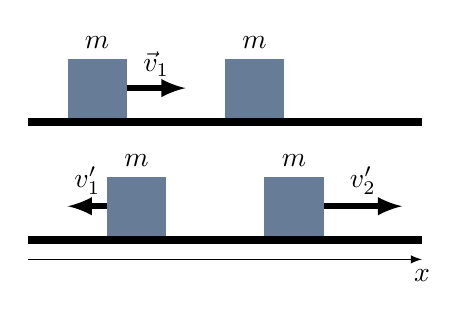
\begin{tikzpicture}
\tikzmath{
\L=5;
\abox=0.75;
}

\scalebox{1}{
\fill (0,-0.1) rectangle (\L,0);

\fill[color=myblue!60] (0.5,0) rectangle +(\abox,\abox);
\fill[color=myblue!60] (2.5,0) rectangle +(\abox,\abox);
\node[above] at (0.5+\abox/2,\abox) {$m$};
\node[above] at (2.5+\abox/2,\abox) {$m$};
\draw[-latex,line width=2] (0.5+\abox,\abox/2) -- +(0.75,0) node[midway,above]{$\vec v_1$};

\begin{scope}[shift={(0,-1.5)}]
\fill (0,-0.1) rectangle (\L,0);
\fill[color=myblue!60] (1,0) rectangle +(\abox,\abox);
\fill[color=myblue!60] (3,0) rectangle +(\abox,\abox);
\node[above] at (1+\abox/2,\abox) {$m$};
\node[above] at (3+\abox/2,\abox) {$m$};
\draw[-latex,line width=2] (1,\abox/2) -- +(-0.5,0) node[midway,above]{$\pvec v'_1$};
\draw[-latex,line width=2] (3+\abox,\abox/2) -- +(1,0) node[midway,above]{$\pvec v'_2$};
\draw[-latex] (0,-0.3) -- +(\L,0) node[below]{$x$};
\end{scope}

}
\end{tikzpicture}
\captionof*{figure}{\textit{A block of mass, $m$, with speed $v_1$, collides elastically with another block of mass, $m$, initially at rest.}}
\end{center}
}


%%%%%%%%%%%%%%%%%%%%%%%%%%%%%%%%
\begin{frame}{Useful trick for elastic collisions}
\begin{itemize}
\item Instead of writing ``before''= ``after'':
\begin{align*}
v_1&= v_1'+v_2'\\
v_1^2&= {v'}_1^{2}+ {v'}_2^{2}
\end{align*}
\item Write ``1'' = ``2'':
\begin{align}
v_1-v_1'&=v_2'\\
v_1^2-{v'}_1^{2}&= {v'}_2^{2}\\
\therefore (v_1-v'_1)(v_1+v'_1)&={v'}_2^{2}\quad\text{(factoring equation 2)}
\end{align}
\item Divide equation 3 by equation 1:
\begin{align*}
\frac{(v_1-v'_1)(v_1+v'_1)}{v_1-v_1'}=v'_2\quad \rightarrow \quad \Aboxed{v_1+v'_1 = v'_2}
\end{align*}
\end{itemize}

\end{frame}


%%%%%%%%%%%%%%%%%%%%%%%%%%%%%%%%
\twocolframesf{Elastic collision in 1D: $m$ collides with $m$ at rest}
{
\begin{itemize}
\item Solve for the final velocities:
\begin{align*}
v_1-v_1'&=v_2'\\
v_1+v'_1 &= v'_2
\end{align*}
\item Which gives:
\begin{align*}
v'_1&=0\\
v'_2&=v_1
\end{align*}
The first block comes to rest and the second one moves with the same speed as the first one did!
\end{itemize}
}
{
\begin{center}
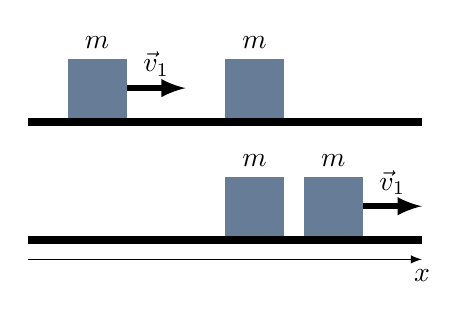
\begin{tikzpicture}
\tikzmath{
\L=5;
\abox=0.75;
}

\scalebox{1}{
\fill (0,-0.1) rectangle (\L,0);

\fill[color=myblue!60] (0.5,0) rectangle +(\abox,\abox);
\fill[color=myblue!60] (2.5,0) rectangle +(\abox,\abox);
\node[above] at (0.5+\abox/2,\abox) {$m$};
\node[above] at (2.5+\abox/2,\abox) {$m$};
\draw[-latex,line width=2] (0.5+\abox,\abox/2) -- +(0.75,0) node[midway,above]{$\vec v_1$};

\begin{scope}[shift={(0,-1.5)}]
\fill (0,-0.1) rectangle (\L,0);
\fill[color=myblue!60] (2.5,0) rectangle +(\abox,\abox);
\fill[color=myblue!60] (3.5,0) rectangle +(\abox,\abox);
\node[above] at (2.5+\abox/2,\abox) {$m$};
\node[above] at (3.5+\abox/2,\abox) {$m$};

\draw[-latex,line width=2] (3.5+\abox,\abox/2) -- +(0.75,0) node[midway,above]{$\vec v_1$};
\draw[-latex] (0,-0.3) -- +(\L,0) node[below]{$x$};
\end{scope}

}
\end{tikzpicture}
\captionof*{figure}{\textit{A block of mass, $m$, with speed $v_1$, collides elastically with another block of mass, $m$, initially at rest.}}
\end{center}
}


%%%%%%%%%%%%%%%%%%%%%%%%%%%%%%%%


%%%%%%%%%%%%%%%%%%%%%%%%%%%%%%%%
\subsection{How to identify an elastic collision}
\label{subsec:howtoidentifyanelasticcollision}
\begin{frame}{How to tell if it is elastic?}
\begin{itemize}
\item Calculate the initial and final kinetic energies and compare them. 
\begin{itemize}
\item Problem solving hint: If you are given enough information to be able to calculate the initial and final velocities using only conservation of momentum, chances are it was inelastic...
\end{itemize}
\item If two objects stick together, or come unstuck (e.g. explosion), then the energy is not conserved:
\begin{itemize}
\item Think of two equal masses coming towards each other at the same speed and coming to rest stuck together. The total momentum is always zero, but the total kinetic energy went from non-zero to zero.
\end{itemize}
\item If you are told about the collision mechanism, you might be able to determine if it’s elastic. E.g. colliding with a spring is elastic (that’s where the term comes from).
\end{itemize}
\end{frame}


%%%%%%%%%%%%%%%%%%%%%%%%%%%%%%%%


%%%%%%%%%%%%%%%%%%%%%%%%%%%%%%%%
\subsection{Example: basketball and tennis ball}
\label{subsec:basketballandtennisball}
\twocolframesf{Basketball and tennis ball}
{

\only<1-2>{
\begin{itemize}
\item Just before the collision,  assume that tennis ball speed = basketball speed. Assume elastic collision (between balls and with the ground).
\item Work it out... you will find:
\begin{align*}
v'_t = \frac{3M-m}{M+m}v
\end{align*}
\item<2-> Re-write as (divide through by $M$):
\begin{align*}
v'_t = \frac{3-\frac{m}{M}}{1+\frac{m}{M}}v
\end{align*}
\item<2-> If $M>>m$, $\frac{m}{M}\sim 0$ and $v'_t\sim 3 v$. 
\end{itemize}
}
\only<3->{
\begin{itemize}
\item<3-> If $M>>m, \frac{m}{M}\sim 0$:
\begin{align*}
v'_t = \frac{3-\frac{m}{M}}{1+\frac{m}{M}}v\sim 3v
\end{align*}
\item<4> With speed $v$, the tennis ball will go a height $h$:
\begin{align*}
mgh&=\frac{1}{2}mv^2\\
\therefore h &\propto v^2
\end{align*}
The height of the bounce goes as speed squared: the tennis ball will bounce to 9$\times$ than from where it was released.
\end{itemize}


}
}
{
\vspace{-1cm}
\begin{center}
\begin{tikzpicture}
\tikzmath{
\h=3;
}

\scalebox{1}{
\node at (0,0) {
\includegraphics[scale=0.5]{figures/MomentumAndCM/bball}};
\node at (0,\h) {
\includegraphics[scale=0.5]{figures/MomentumAndCM/tball}};
\draw[-latex, line width=1.5] (0,\h) -- +(0,-1) node[midway,right]{$-\vec v$};
\draw[-latex, line width=1.5] (0,0.75) -- +(0,1) node[left]{$\vec v$};

\begin{scope}[shift={(2,0)}]
\node at (0,0) {
\includegraphics[scale=0.5]{figures/MomentumAndCM/bball}};
\node at (0,\h) {
\includegraphics[scale=0.5]{figures/MomentumAndCM/tball}};
\draw[-latex, line width=1.5] (0,\h) -- +(0,2) node[left]{$\pvec v'_t$};
\draw[-latex, line width=1.5] (0,0.75) -- +(0,1) node[left]{$\pvec v'_b$};
\end{scope}
}
\end{tikzpicture}
\captionof*{figure}{\textit{A basketball colliding with a tennis ball.}}
\end{center}
}


%%%%%%%%%%%%%%%%%%%%%%%%%%%%%%%%
\subsection{Ballistic pendum}
\label{subsec:ballisticpendulum}
\twocolframesf{Ballistic pendulum}
{
\begin{itemize}
\item The bullet/arrow embeds itself in the pendulum block.
\item The pendulum rises.
\item The height allows you to determine the speed of the arrow.
\end{itemize}
}
{
\begin{center}
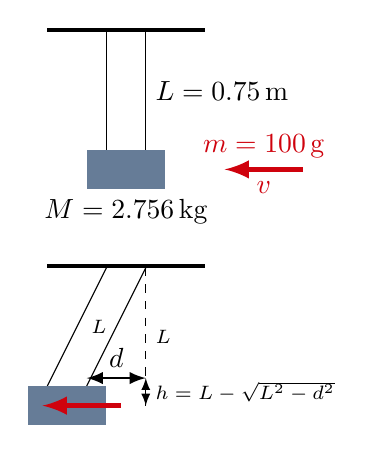
\begin{tikzpicture}
\tikzmath{
\Lc=2;
\L=1.5;
\h=0.25;
\boxh=0.5;
\boxL=1;
\ropew=0.5*\boxL;
\dis=0.75;
}

\scalebox{1}{

\fill (-\Lc/2,0) rectangle (\Lc/2,0.05);
\draw (-\ropew/2,0) -- +(0,-\L);
\draw (\ropew/2,0) -- +(0,-\L) node[midway,right]{$L=\SI{0.75}{m}$};
\fill[color=myblue!60] (-\boxL/2,-\L) rectangle (\boxL/2,-\L-\boxh);
\draw[color=myred, line width=2,latex-] (\boxL/2+\dis,-\L-\boxh/2) -- +(1,0) node[midway,above]{$m=\SI{100}{g}$}node[midway,below]{$v$};
\node[below] at (0,-\L-\boxh) {$M=\SI{2.756}{kg}$};

\begin{scope}[shift={(0,-3)}]
\fill (-\Lc/2,0) rectangle (\Lc/2,0.05);
\draw (-\ropew/2,0) -- +(-\dis,-\L);
\draw (\ropew/2,0) -- +(-\dis,-\L) node[midway,left]{\scriptsize $L$};

\fill[color=myblue!60] (-\boxL/2-\dis,-\L) rectangle (\boxL/2-\dis,-\L-\boxh);
\draw[color=myred, line width=2,latex-] (-\boxL/2-0.75*\dis,-\L-\boxh/2) -- +(1,0) ;

\draw[dashed] (\ropew/2,0) -- +(0,-\L-\h) node[midway,right]{\scriptsize $L$};
\draw[latex-latex, line width=1] (\ropew/2,-\L+0.1) -- +(-\dis,0) node[midway,above]{$d$};
\draw[latex-latex, line width=0.5] (\ropew/2,-\L-\h) -- +(0,0.1+\h) node[midway,right]{\scriptsize $h=L-\sqrt{L^2-d^2}$};
\end{scope}

}
\end{tikzpicture}
\captionof*{figure}{\textit{An arrow embeds itself into a ballistic pendulum.}}
\end{center}
}


%%%%%%%%%%%%%%%%%%%%%%%%%%%%%%%%

%%%%%%%%%%%%%%%%%%%%%%%%%%%%%%%%
\twocolframesf{Exercise: Find the speed of the arrow, given $d$.}
{
\begin{itemize}
\item<2-> Conservation of momentum (inelastic collision):
\begin{align*}
mv=(M+m)v'
\end{align*}
\item<3-> Conservation of energy after the collision:
\begin{align*}
\frac{1}{2}(M+m){v'}^2=(M+m)gh
\end{align*}
\item<4-> You should find:
\begin{align*}
v &= \frac{M+m}{m}\sqrt{2g\left(L-\sqrt{L^2-d^2}\right)}\\
&= (28.56)\sqrt{(\SI{19.6}{m/s^2})\left((\SI{0.75}{m})-\sqrt{(\SI{0.75}{m})^2-d^2}\right)}
\end{align*}
\end{itemize}
}
{
\begin{center}
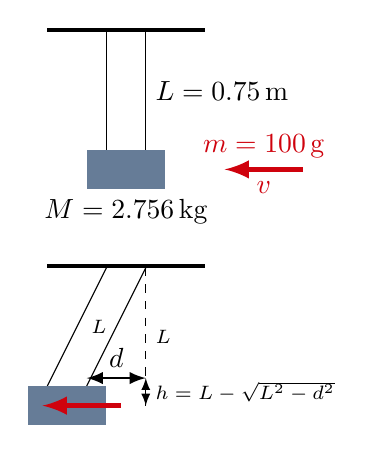
\begin{tikzpicture}
\tikzmath{
\Lc=2;
\L=1.5;
\h=0.25;
\boxh=0.5;
\boxL=1;
\ropew=0.5*\boxL;
\dis=0.75;
}

\scalebox{1}{

\fill (-\Lc/2,0) rectangle (\Lc/2,0.05);
\draw (-\ropew/2,0) -- +(0,-\L);
\draw (\ropew/2,0) -- +(0,-\L) node[midway,right]{$L=\SI{0.75}{m}$};
\fill[color=myblue!60] (-\boxL/2,-\L) rectangle (\boxL/2,-\L-\boxh);
\draw[color=myred, line width=2,latex-] (\boxL/2+\dis,-\L-\boxh/2) -- +(1,0) node[midway,above]{$m=\SI{100}{g}$} node[midway,below]{$v$};
\node[below] at (0,-\L-\boxh) {$M=\SI{2.756}{kg}$};

\begin{scope}[shift={(0,-3)}]
\fill (-\Lc/2,0) rectangle (\Lc/2,0.05);
\draw (-\ropew/2,0) -- +(-\dis,-\L);
\draw (\ropew/2,0) -- +(-\dis,-\L) node[midway,left]{\scriptsize $L$};

\fill[color=myblue!60] (-\boxL/2-\dis,-\L) rectangle (\boxL/2-\dis,-\L-\boxh);
\draw[color=myred, line width=2,latex-] (-\boxL/2-0.75*\dis,-\L-\boxh/2) -- +(1,0) ;

\draw[dashed] (\ropew/2,0) -- +(0,-\L-\h) node[midway,right]{\scriptsize $L$};
\draw[latex-latex, line width=1] (\ropew/2,-\L+0.1) -- +(-\dis,0) node[midway,above]{$d$};
\draw[latex-latex, line width=0.5] (\ropew/2,-\L-\h) -- +(0,0.1+\h) node[midway,right]{\scriptsize $h=L-\sqrt{L^2-d^2}$};
\end{scope}

}
\end{tikzpicture}
\captionof*{figure}{\textit{An arrow embeds itself into a ballistic pendulum.}}
\end{center}
}

%%%%%%%%%%%%%%%%%%%%%%%%%%%%%%%%








%%%%%%%%%%%%%%%%%%%%%%%%%%%%%%%%
\section{Centre of Mass}
\label{sec:centreofmass}
\title{Centre of Mass}
\institute{Momentum and Centre of Mass}
\author{\insertsubsection}


%%%%%%%%%%%%%%%%%%%%%%%%%
\begin{frame}
\titlepage
\thispagestyle{empty}
\end{frame}

%%%%%%%%%%%%%%









%%%%%%%%%%%%%%%%%%%%%%%%%%%%%%%%
\subsection{Describing a system}
\label{subsec:describingasystem}
\begin{frame}{Describing a system}
\begin{itemize}
\item We can define a system of particles; that system can be particles that are freely moving with respect to each other, or it could be a solid object.
\item We found that the motion of the system as a whole is determined by the external forces on the system (the internal forces cancel out).
\item Want to define some quantities that allow us to describe the motion of the system as a whole:
\begin{itemize}
\item Total momentum $\rightarrow$ add momenta of particles in the system.
\item Total energy (kinetic + potential) $\rightarrow$ add energies of particles in the system.
\item Position $\rightarrow$ figure out some average position of the system (the CM).
\end{itemize}

\end{itemize}

\end{frame}


%%%%%%%%%%%%%%%%%%%%%%%%%%%%%%%%
\twocolframesf{Describing a system}
{
\begin{itemize}
\item The total momentum of a system:
\begin{align*}
\vec P=\vec p_1 + \vec p_2 + \vec p_3 + \dots
\end{align*}
is conserved if there are no net external forces:
\begin{align*}
\frac{d\vec P}{dt}=\sum_{system} \vec F^{ext}
\end{align*}
\item Want to write Newton’s 2nd Law, using the \textbf{total mass of the system}, $M$:
\begin{align*}
\sum_{system} \vec F^{ext}=M\vec a_{CM}
\end{align*}

\item But, $a_{CM}$, is the acceleration of what??

\end{itemize}
}
{
\vspace{-1cm}
\begin{center}
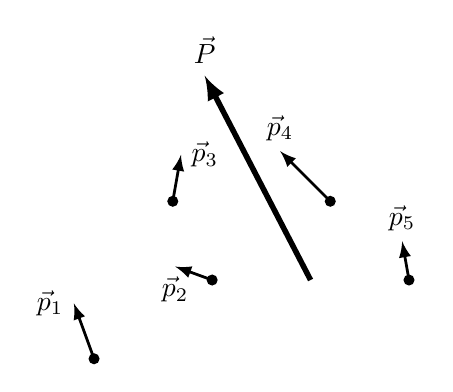
\begin{tikzpicture}

\scalebox{1}{

\coordinate (P1) at (0,0);
\coordinate (P2) at (1.5,1);
\coordinate (P3) at (1,2);
\coordinate (P4) at (3,2);
\coordinate (P5) at (4,1);
\coordinate (P) at (2.75,1);
\fill (P1) circle (2pt);
\fill (P2) circle (2pt);
\fill (P3) circle (2pt);
\fill (P4) circle (2pt);
\fill (P5) circle (2pt);

\draw[-latex, line width=1] (P1) -- +(110:0.75) node[left]{$\vec p_1$};
\draw[-latex, line width=1] (P2) -- +(160:0.5) node[below]{$\vec p_2$};
\draw[-latex, line width=1] (P3) -- +(80:0.6) node[right]{$\vec p_3$};
\draw[-latex, line width=1] (P4) -- +(135:0.9) node[above]{$\vec p_4$};
\draw[-latex, line width=1] (P5) -- +(100:0.5) node[above]{$\vec p_5$};

\draw[-latex, line width=2] (P) -- ($(P)+(110:0.75)+(160:0.5)+(80:0.6)+(135:0.9)+(100:0.5)$) node[above]{$\vec P$};
}
\end{tikzpicture}
\captionof*{figure}{\textit{The momentum of a system of particles is given by the sum of the individual momenta of the particles.}}
\end{center}
\scriptsize
For one particle:
\begin{align*}
\frac{d\vec p_i}{dt}=\sum \vec F=m\vec a = m\frac{d\vec v}{dt}=m\frac{d^2\vec r}{dt^2}
\end{align*}
}


%%%%%%%%%%%%%%%%%%%%%%%%%%%%%%%%
\subsection{Concept}
\label{subsec:conceptcm}
\begin{frame}{Centre of mass}
\begin{itemize}
\item We define the centre of mass of a system to be that \textbf{location in the system that is described by}:
\begin{align*}
\sum_{system} \vec F^{ext}=M\vec a_{CM}
\end{align*}
\item That is, within the system, there exist a point, whose position, $\vec r_{CM}$ is such that:
\begin{align*}
\vec a_{CM}=\frac{d^2\vec r}{dt^2}
\end{align*}
\item The centre of mass is that position in the system that moves according to Newton’s Second Law, where:
\begin{itemize}
\item $M$ is the total mass of the system.
\item $\sum_{system} \vec F^{ext}$ is the sum over external forces exerted on the system.
\end{itemize}

\end{itemize}
\end{frame}


%%%%%%%%%%%%%%%%%%%%%%%%%%%%%%%%


%%%%%%%%%%%%%%%%%%%%%%%%%%%%%%%%
\subsubsection{CM location}
\label{subsubsec:cmlocation}
\twocolframesf{Location of the centre of mass}
{
\begin{itemize}
\item Weighted sum of the positions of each particle in the system:
\begin{align*}
\vec r_{CM}=\frac{1}{M}\sum m_i \vec r_i
\end{align*}
\item Vector equation, so true for each component:
\begin{align*}
x_{CM}&=\frac{1}{M}\sum m_i x_i\\
y_{CM}&=\frac{1}{M}\sum m_i y_i\\
z_{CM}&=\frac{1}{M}\sum m_i z_i
\end{align*}
\end{itemize}
}{
\vspace{-1cm}
\begin{center}
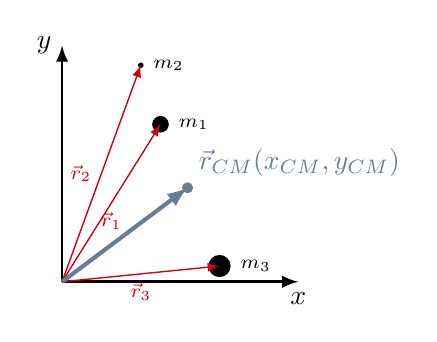
\begin{tikzpicture}

\scalebox{1}{
\draw[-latex, line width=1] (0,0)--(3,0) node[below]{$x$};
\draw[-latex, line width=1] (0,0)--(0,3) node[left]{$y$};

\coordinate (P1) at (1.25,2);
\coordinate (P2) at (1,2.75);
\coordinate (P3) at (2,0.2);

\fill (P1) circle (3pt) node[right=3pt]{\scriptsize $m_1$};
\fill (P2) circle (1pt) node[right=1pt]{\scriptsize $m_2$};
\fill (P3) circle (4pt) node[right=4pt]{\scriptsize $m_3$};

\draw[-latex, line width=0.5,color=myred] (0,0) -- (P1) node[midway,below]{\scriptsize $\vec r_1$};
\draw[-latex, line width=0.5,color=myred] (0,0) -- (P2) node[midway,left]{\scriptsize $\vec r_2$};
\draw[-latex, line width=0.5,color=myred] (0,0) -- (P3) node[midway,below]{\scriptsize $\vec r_3$};

\draw[-latex, line width=1.5,color=myblue!60] (0,0) -- +($3/8*(P1)+1/8*(P2)+0.5*(P3) $) node[above right]{$\vec r_{CM}(x_{CM},y_{CM})$};
\fill[color=myblue!60] ($3/8*(P1)+1/8*(P2)+0.5*(P3) $) circle(2pt);
}
\end{tikzpicture}
\captionof*{figure}{\textit{The centre of mass of particles in a system is that point of the system that moves according to Newton's Laws applied to the system as a whole.}}
\end{center}
\scriptsize
For example:
\begin{align*}
x_{CM}=\frac{m_1x_1+m_2x_2+m_3x_3}{m_1+m_2+m_3}
\end{align*}
}


%%%%%%%%%%%%%%%%%%%%%%%%%%%%%%%%


%%%%%%%%%%%%%%%%%%%%%%%%%%%%%%%%
\subsubsection{CM velocity}
\label{subsubsec:cmvelocity}
\begin{frame}{Velocity and acceleration of CM}
\begin{itemize}
\item By using the CM, we can model a system/object \textit{as if it were a point particle} of mass $M$ located at the centre of mass.
\item The position of that particle moves with (velocity, acceleration):
\begin{align*}
\vec v_{CM}&=\frac{d}{dt} \vec r_{CM}= \frac{1}{M}\sum m_i \vec v_i\\
\vec a_{CM}&=\frac{d}{dt} \vec v_{CM}=\frac{1}{M}\sum m_i \vec a_i
\end{align*}
\end{itemize}
\end{frame}


%%%%%%%%%%%%%%%%%%%%%%%%%%%%%%%%
\subsubsection{CM reference frame}
\label{subsubsec:cmreferenceframe}
\twocolframesf{Collisions as viewed in CM frame of reference}
{
\begin{itemize}
\item In the centre of mass frame of reference, the total momentum of the system is zero, since the velocity of the system in that frame is zero.
\item This is sometimes useful for modeling elastic collisions:\\
As viewed in the CM frame, two particles are momentarily at rest at the instant when they collide and the kinetic energy is correspondingly zero at that time. 
\end{itemize}
}
{
\begin{center}
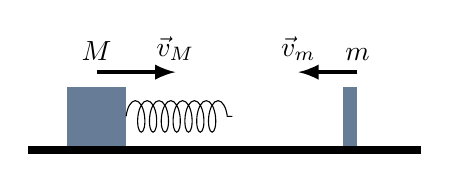
\begin{tikzpicture}
\tikzmath{
\L=5;
\abox=0.75;
}
\scalebox{1}{

\fill (0,-0.1) rectangle (\L,0);

\fill[color=myblue!60] (0.1*\L,0) rectangle +(\abox,\abox);
\fill[color=myblue!60] (0.8*\L,0) rectangle +(\abox/4,\abox);

\draw[-latex, line width=1.5] (0.1*\L+0.5*\abox,1.25*\abox) node[above]{$M$} -- +(1,0) node[above]{$\vec v_M$};
\draw[-latex, line width=1.5] (0.8*\L+0.25*\abox,1.25*\abox) node[above]{$m$} -- +(-0.75,0) node[above]{$\vec v_m$};
\draw[decoration={aspect=0.4, segment length=1.5mm, amplitude=2mm,coil},decorate] (0.1*\L+\abox,0.5*\abox) -- +(0.27*\L,0);
}
\end{tikzpicture}
\captionof*{figure}{\textit{Problem from end of chapter 10. Finding the maximal compression of the spring is difficult in the lab frame. In the CM frame, it is when both blocks come to rest and all of the initial kinetic energy (evaluated in the CM frame) is equal to the potential energy stored in the spring.}}
\end{center}
}


%%%%%%%%%%%%%%%%%%%%%%%%%%%%%%%%
\subsection{CM for a continuous object}
\label{subsec:cmforacontinuousobject}
\twocolframesf{Centre of mass for a continuous object}
{
\vspace{-0.25cm}
\begin{itemize}
\item Model a rod as being made of many mass elements, $\Delta m$, with length, $\Delta x$, each at position, $x_i$:
\begin{align*}
x_{CM}=\frac{1}{M}\sum x_i\Delta m
\end{align*} 
\item The mass of one rod element is:
\begin{align*}
\Delta m = \lambda \Delta x
\end{align*}
where  $\lambda$ is the linear mass density of the rod:
\begin{align*}
\lambda &= \frac{M}{L}\\
\therefore x_{CM}&=\frac{1}{M} \sum \lambda x_i \Delta x
\end{align*}
\end{itemize}
}
{
\begin{center}
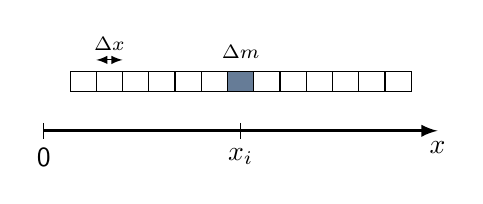
\begin{tikzpicture}
\tikzmath{
\L=5;
\abox=0.75;
\n=15;
}
\scalebox{1}{

\draw[-latex,line width=1] (0,0) -- (\L,0) node[below]{$x$};
\draw (0,0.1) -- +(0,-0.2) node[below]{0};

\foreach \i in {1,...,13}{
\tikzmath{
\dx=\L/\n;
\xxi=\dx*\i;
}
\draw (\xxi,0.5) rectangle (\xxi+\dx,0.75);
\ifthenelse{\i=7}{
\fill[color=myblue!60] (\xxi,0.5) rectangle (\xxi+\dx,0.75);
\node at (\xxi+0.5*\dx,1) {\scriptsize $\Delta m$};
\draw (\xxi+0.5*\dx,0.1) -- +(0,-0.2) node[below]{$x_i$};
}{}

\ifthenelse{\i=2}{
\draw[latex-latex] (\xxi,0.9) -- +(0\dx,0) node[midway,above]{\scriptsize $\Delta x$};
}{}

}


}
\end{tikzpicture}
\captionof*{figure}{\textit{To find the CM of a one dimensional object, model it as being made of many \textit{point} masses, $\Delta m$, each with an infinitesimal length, $\Delta x$.}}
\end{center}
}

%%%%%%%%%%%%%%%%%%%%%%%%%%%%%%%%


%%%%%%%%%%%%%%%%%%%%%%%%%%%%%%%%
\twocolframesf{Centre of mass for a continuous object}
{
\vspace{-0.25cm}
\begin{itemize}
\item Model a rod as being made of many mass elements, $\Delta m$, with length, $\Delta x$, each at position, $x_i$:
\begin{align*}
x_{CM}=\frac{1}{M}\sum x_i\Delta m
\end{align*} 
\item The mass of one rod element is:
\begin{align*}
\Delta m = \lambda \Delta x
\end{align*}
where  $\lambda$ is the linear mass density of the rod:
\begin{align*}
\lambda &= \frac{M}{L}\\
\therefore x_{CM}&=\frac{1}{M} \sum \lambda x_i \Delta x
\end{align*}
\end{itemize}
}
{
\begin{center}
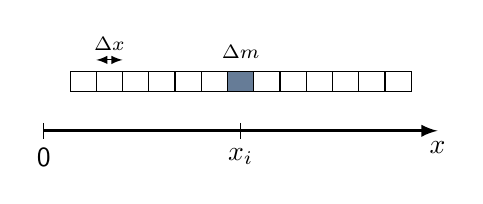
\begin{tikzpicture}
\tikzmath{
\L=5;
\abox=0.75;
\n=15;
}
\scalebox{1}{

\draw[-latex,line width=1] (0,0) -- (\L,0) node[below]{$x$};
\draw (0,0.1) -- +(0,-0.2) node[below]{0};

\foreach \i in {1,...,13}{
\tikzmath{
\dx=\L/\n;
\xxi=\dx*\i;
}
\draw (\xxi,0.5) rectangle (\xxi+\dx,0.75);
\ifthenelse{\i=7}{
\fill[color=myblue!60] (\xxi,0.5) rectangle (\xxi+\dx,0.75);
\node at (\xxi+0.5*\dx,1) {\scriptsize $\Delta m$};
\draw (\xxi+0.5*\dx,0.1) -- +(0,-0.2) node[below]{$x_i$};
}{}

\ifthenelse{\i=2}{
\draw[latex-latex] (\xxi,0.9) -- +(0\dx,0) node[midway,above]{\scriptsize $\Delta x$};
}{}

}


}
\end{tikzpicture}
\captionof*{figure}{\textit{To find the CM of a one dimensional object, model it as being made of many \textit{point} masses, $\Delta m$, each with an infinitesimal length, $\Delta x$.}}
\end{center}
If $\lambda$ is constant:
\begin{align*}
x_{CM}&=\frac{1}{M}\int_0^L\lambda x dx \\
&= \frac{1}{M}\frac{1}{2}\lambda L^2 = \frac{1}{M}\frac{1}{2}\frac{M}{L}L^2=\frac{1}{2}L
\end{align*}
}



%%%%%%%%%%%%%%%%%%%%%%%%%%%%%%%%
\twocolframesf{Centre of mass for a continuous object}
{
\vspace{-0.25cm}
\begin{align*}
x_{CM}&=\frac{1}{M}\int_0^M x dm\\
y_{CM}&=\frac{1}{M}\int_0^M y dm\\
z_{CM}&=\frac{1}{M}\int_0^M z dm
\end{align*}
where $dm$ is a small mass element at position $(x,y,z)$.
\begin{itemize}
\item Strategy:
\begin{itemize}
\item Express $dm$ in terms of a density and a \textbf{position} coordinate.
\item \textcolor{myred}{Limits of the integral} correspond to range of coordinates of the object.
\end{itemize}

\end{itemize}
}
{
\vspace{-1cm}
\begin{center}
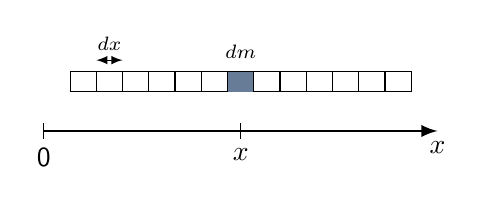
\begin{tikzpicture}
\tikzmath{
\L=5;
\abox=0.75;
\n=15;
}
\scalebox{1}{

\draw[-latex,line width=1] (0,0) -- (\L,0) node[below]{$x$};
\draw (0,0.1) -- +(0,-0.2) node[below]{0};
\foreach \i in {1,...,13}{
\tikzmath{
\dx=\L/\n;
\xxi=\dx*\i;
}
\draw (\xxi,0.5) rectangle (\xxi+\dx,0.75);
\ifthenelse{\i=7}{
\fill[color=myblue!60] (\xxi,0.5) rectangle (\xxi+\dx,0.75);
\node at (\xxi+0.5*\dx,1) {\scriptsize $dm$};
\draw (\xxi+0.5*\dx,0.1) -- +(0,-0.2) node[below]{$x$};
}{}

\ifthenelse{\i=2}{
\draw[latex-latex] (\xxi,0.9) -- +(\dx,0) node[midway,above]{\scriptsize $dx$};
}{}
}
}
\end{tikzpicture}
\captionof*{figure}{\textit{To find the CM of a one dimensional object, model it as being made of many \textit{point} masses, $\Delta m$, each with an infinitesimal length, $\Delta x$.}}
\end{center}
Given linear mass density, $\lambda$:
\begin{align*}
dm&=\lambda dx \;\;\text{(change of variables)}\\
x_{CM}&=\frac{1}{M}\int_{\textcolor{myred}{0}}^{\textcolor{myred}{M}} x dm=\frac{1}{M}\int_{\textcolor{myred}{0}}^{\textcolor{myred}{L}} x \lambda dx\\
M&=\int_{\textcolor{myred}{0}}^{\textcolor{myred}{M}} dm=\int_{\textcolor{myred}{0}}^{\textcolor{myred}{L}} \lambda dx
\end{align*}
}


%%%%%%%%%%%%%%%%%%%%%%%%%%%%%%%%


%%%%%%%%%%%%%%%%%%%%%%%%%%%%%%%%
\subsection{CM of a sqaure}
\label{subsec:cmofasquare}
\twocolframesf{CM of continuous 2D object (square)}
{
\begin{itemize}
\item<2-> Break up the object of dimension D into infinitesimal mass elements of dimension D-1:
\begin{itemize}
	\item[$\rightarrow$] A square is a sum of rods.
\end{itemize}
\item<3-> Identify the CM of the object of dimension D-1:
\begin{itemize}
	\item[$\rightarrow$] CM of rods is their centre.
\end{itemize}
\item<4-> Write the mass of the mass element using \textbf{surface mass density}, $\sigma$:
\begin{align*}
dm=\sigma dA = \sigma a dy=\frac{M}{a^2}ady=\frac{M}{a}dy
\end{align*}
\item<5-> Solve for the CM:
\begin{align*}
y_{CM}&=\frac{1}{M}\int_0^M y dm=\frac{1}{M}\int_0^a y \frac{M}{a}dy=\frac{1}{2}a
\end{align*}
\end{itemize}
}
{
\begin{center}
\begin{tikzpicture}
\tikzmath{
\L=3;
\dy=0.4;
}
\scalebox{1}{
%object
\fill[color=myblue!30] (0,0) rectangle (\L,\L);
\node[above] at (0.5*\L,\L){$a$};

\only<2->{
%strip
\fill[color=myblue!60] (0,0.25*\L) rectangle (\L,0.25*\L+\dy);

\draw[latex-latex] (\L+0.1,0.25*\L) -- (\L+0.1,0.25*\L+\dy) node[midway,right] {\scriptsize $dy$};

\only<3->{
\fill (0.5*\L,0.25*\L+0.5*\dy) circle(3pt);
}
\only<4->{
\node[above] at (0.5*\L,0.25*\L+\dy) {$dm$};
\node[below] at (0.5*\L,0.25*\L) {$dA=ady$};
}
}
\draw[-latex,line width=1.5] (0,0) -- (1.3*\L,0) node[below]{$x$};
\draw[-latex,line width=1.5] (0,0) -- (0,1.3*\L) node[left]{$y$};
}
\end{tikzpicture}
\captionof*{figure}{\textit{To find the CM of a two dimensional object, model it as being made of many 1 dimensional objects (e.g. rods) each with mass $dm$.}}
\end{center}
}

%%%%%%%%%%%%%%%%%%%%%%%%%%%%%%%%
\subsection{CM of a triangle}
\label{subsec:cmofatriangle}
\twocolframesf{CM of continuous 2D object (isosceles triangle)}
{
\begin{itemize}
\item For an isosceles ($L$, $h$) triangle of mass $M$:
\begin{itemize}
\item What is the surface mass density?
\only<2->{
\begin{align*}
\sigma=\frac{M}{A}=\frac{M}{\frac{1}{2}Lh}=\frac{2M}{Lh}
\end{align*}
}
\item What is the mass of a little rod at position $y$?
\only<3->{
\begin{align*}
dm&=\sigma dA=\sigma D(y) dy\\
D(0)&=0\;\;D(h)=L\;\;\rightarrow\;\;D(y)=\frac{L}{h}y
\end{align*}
}
\item What is the integral for the CM?
\only<4->{
\begin{align*}
y_{CM}&=\frac{1}{M}\int_0^M y dm=\frac{1}{M}\int_0^h \sigma \frac{L}{h}y^2 dy
\end{align*}
}
\end{itemize}

\end{itemize}
}
{
\begin{center}
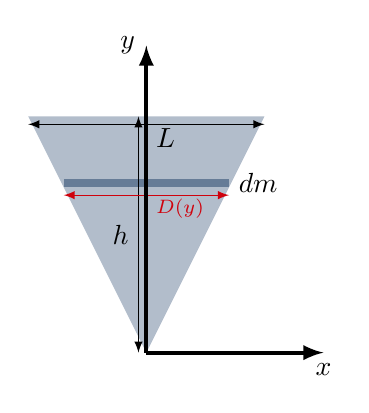
\begin{tikzpicture}
\tikzmath{
\L=3;
\h=3;
\dy=0.1;
\hy=\L/2/\h*0.7*\L;
}
\scalebox{1}{
%object
\fill[color=myblue!30] (0,0) -- (\L/2,\h) -- (-\L/2,\h) -- cycle;


%strip
\fill[color=myblue!60] (-\hy,0.7*\h) rectangle (\hy,0.7*\h+\dy);
\node[right] at (\hy,0.7*\h+0.5*\dy){$dm$};


\draw [latex-latex] (-0.1,0) -- +(0,\h) node[midway,left]{$h$};
\draw [latex-latex] (-\L/2,\h-0.1) -- +(\L,0) node[midway,below=5pt, right]{$L$};

\draw [latex-latex,color=myred] (-\hy,0.7*\h-0.1) -- (\hy,0.7*\h-0.1) node[midway,below=5pt, right]{\scriptsize $D(y)$};

\draw[-latex,line width=1.5] (0,0) -- (0.75*\L,0) node[below]{$x$};
\draw[-latex,line width=1.5] (0,0) -- (0,1.3*\h) node[left]{$y$};
}
\end{tikzpicture}
\captionof*{figure}{\textit{To find the CM of a two dimensional object, model it as being made of many 1 dimensional objects (e.g. rods) each with mass $dm$.}}
\end{center}
}


%%%%%%%%%%%%%%%%%%%%%%%%%%%%%%%%
\subsection{CM of a 3D object}
\label{subsec:cmofa3dobject}
\twocolframesf{CM of continuous 3D object (parabolic volume of height, $h$)}
{
\begin{itemize}
\scriptsize
\item Given the volume density, $\rho$ (don’t know the mass).
\item Need radius as a function of height, $r(z)$:
\begin{align*}
z\propto r^2 \;\;\rightarrow\;\;r(z)=a\sqrt{z}
\end{align*}

\item Model as small disks of radius, $r(z)$, and height, $dz$:
\begin{align*}
dm=\rho dV = \rho \pi r^2(z) dz=\rho \pi a^2 z dz
\end{align*}
\item The integral for the CM:
\begin{align*}
z_{CM}&=\frac{1}{M}\int_0^M z dm=\frac{1}{M}\int_0^h \rho\pi a^2z^2 dz
\end{align*}
\item The total mass:
\begin{align*}
M&=\frac{1}{M}\int_0^M dm=\int_0^h \rho\pi a^2z dz
\end{align*}
\end{itemize}
}
{
\begin{center}
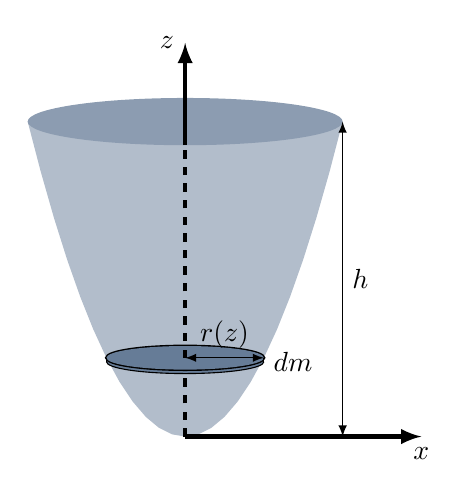
\begin{tikzpicture}
\tikzmath{
\h=3;
}
\scalebox{1}{
\fill[domain = -2:2, variable = \x, color=myblue!30] plot ({\x},{\x*\x});
\fill[color=myblue!45] (0,4) circle (2 and 0.3);

\draw[-latex,line width=1.5] (0,0) -- (3,0) node[below]{$x$};

\draw[line width=1.5, dashed] (0,0) -- (0,0.85) ;
\begin{scope}[shift={(0,-0.05)}]
\fill[color=myblue!60] (0,1) circle (1 and 0.15);
\draw (1,1) arc (0:-180:1 and 0.15);
\end{scope}
\draw[line width=1] (0,1) circle (1 and 0.15);
\fill[color=myblue!60] (0,1) circle (1 and 0.15);
\draw (1,1) -- +(0,-0.05)node[right]{$dm$};
\draw[latex-latex] (0,1) -- (1,1) node[midway,above]{$r(z)$};
\draw (-1,1) -- +(0,-0.05);
\draw[line width=1.5, dashed] (0,1) -- (0,3.7);
\draw[-latex,line width=1.5] (0,3.7) -- (0,5) node[left]{$z$};

\draw[latex-latex] (2,0) -- (2,4) node[midway,right]{$h$};

}
\end{tikzpicture}
\captionof*{figure}{\textit{Model the parabolic volume as made of disks. $y$ is into the page.}}
\end{center}
}



%%%%%%%%%%%%%%%%%%%%%%%%%%%%%%%%



%%%%%%%%%%%%%%%%%%%%%%%%%%%%%%%%



%%%%%%%%%%%%%%%%%%%%%%%%%%%%%%%%



%%%%%%%%%%%%%%%%%%%%%%%%%%%%%%%%



%%%%%%%%%%%%%%%%%%%%%%%%%%%%%%%%



%%%%%%%%%%%%%%%%%%%%%%%%%%%%%%%%



%%%%%%%%%%%%%%%%%%%%%%%%%%%%%%%%



%%%%%%%%%%%%%%%%%%%%%%%%%%%%%%%%



%%%%%%%%%%%%%%%%%%%%%%%%%%%%%%%%



%%%%%%%%%%%%%%%%%%%%%%%%%%%%%%%%



%%%%%%%%%%%%%%%%%%%%%%%%%%%%%%%%



%%%%%%%%%%%%%%%%%%%%%%%%%%%%%%%%



%%%%%%%%%%%%%%%%%%%%%%%%%%%%%%%%






\end{document}
